% Usage: knitr slide

%
%### One sample/Paired: Modification of Student's sleep data ###%
%
%d1 <- sleep$extra[sleep$group==2] - sleep$extra[sleep$group==1]
%d1[1] <- d1[1] * -1

\chapter{Nonparametric Statistical Tests}\alabel{chap:nonpar}\ros{9}\katz{5.4}\bmovie{10}\ddisc{10}
\section{When to use non-parametric methods}
\bi
\item Short answer: Good default when $P$-values are needed and there are no covariates to adjust for
\item Nonparametric methods are those not requiring one to assume a
  certain distribution for the raw data
  \bi
  \item In contrast, parametric methods assume data come from some underlying distribution
  \item $t$-tests assume the data come form a Gaussian distribution
  \ei
\item Response variable ordinal or interval
\item For ordinal responses nonparametric methods are preferred
  because they assume no spacing between categories
\item No problem in using nonparametric tests on interval data
 \bi
 \item if normality holds, nonpar.\ test 0.95 efficient, i.e., has
   about the same power as the parametric test done on 0.95 of the
   observations\footnote{The large-sample efficiency of the Wilcoxon
     and Spearman tests compared to $t$ and $r$ tests is
     $\frac{3}{\pi} = 0.9549$.}
 \item if normality does not hold, nonpar.\ tests can be arbitrarily
   more efficient and powerful than the corresponding parametric test 
 \item an elegant and non-arbitrary way to deal with extreme values or
   outliers
 \item rank-based nonparametric tests give the analyst freedom from
   having to choose the correct transformation of the measurement (as
   long as the optimum transformation is monotonic)
 \ei
\item Nonparametric methods are robust, many parametric methods are
  not
 \bi
 \item Example: $t$-test comparing two sets of measurements\\
   1 2 3 4 5 6 7 8 9 10 \hfill vs.\ \hfill 7 8 9 10 11 12 13 14 15 16
   17 18 19 20\\
   means: 5.5 and 13.5, $P=0.000019$\\
   1 2 3 4 5 6 7 8 9 10 \hfill vs.\ \hfill 7 8 9 10 11 12 13 14 15 16
   17 18 19 20 \textbf{200}\\
   means: 5.5 and 25.9, $P=0.12$\\
   The SD is a particularly non-robust statistical estimator.
  \ei

\item Example: Fecal calprotectin being evaluated as a possible
  biomarker of disease severity (Figure \ref{fig:nonpar-calpro})
 \bi 
  \item Calprotectin has an upper detection limit
  \item Median can be calculated (mean cannot)
 \ei
\item If all you want is a $P$-value nonpar.\ tests are preferred
 \bi
 \item Especially if response is univariate and no need to adjust for
   covariates
 \ei
\item Pre-testing for normality and deciding nonparametric
  vs.\ parametric analysis is a bad idea
 \bi
 \item Tests for normality do not have a power of 1.0 and type I error
   of 0.0
 \item Leads to temptation, e.g., an investigator might ``forget'' to do the
   test of normality if the $t$-test is significant
 \item Doesn't acknowledge that nonparametric tests are very efficient
   even under normality
 \item Pre-testing for normality alters the type I error and confidence interval coverage
 \ei
\item A drawback is that nonpar.\ tests do not correspond to
  usual confidence limits for effects
 \bi
  \item E.g., a CL for the difference in 2 means may include zero whereas
  the Wilcoxon test yields $P=0.01$
  \item Point estimate that exactly corresponds to the Wilcoxon
    two-sample test is the Hodges-Lehman estimate of the location
    difference
  \bi
  \item median of all possible differences between a measurement from
    group 1 and a measurement from group 2
  \ei
 \ei
\item Nonparametric tests are often obtained by replacing the data
  with ranks across subjects and then doing the parametric test
\item Many nonpar.\ tests give the same $P$-value regardless of how
  the data are transformed; a careful choice of transformation (e.g.,
  log) must sometimes be used in the context of parametric tests
\item $P$-values computed using e.g.\ the $t$ distribution are quite
  accurate for nonparametric tests
\item In case of ties, midranks are used, e.g., if the raw data were
  105 120 120 121 the ranks would be 1 2.5 2.5 4

\begin{center}
\begin{tabular}{lll} \hline
Parametric Test & Nonparametric Counterpart & Semiparametric Model \\
                &                           & Counterpart \\ \hline
1-sample $t$    & Wilcoxon signed-rank & \\
2-sample $t$    & Wilcoxon 2-sample rank-sum & Proportional odds \\
$k$-sample ANOVA           & Kruskal-Wallis  & Proportional odds \\
Pearson $r$     & Spearman $\rho$ & \\ \hline
\end{tabular}\end{center}
\ei

\section{One Sample Test: Wilcoxon Signed-Rank} \ros{9.3}\katz{5.10.E}
\bi
\item Almost always used on paired data where the column of values
  represents differences (e.g., post-pre) or log ratios
\item The \emph{sign test} is the simplest test for the median
  difference being zero in the population
 \bi
 \item it just counts the number of positive differences after tossing
   out zero differences
 \item tests $H_{0}:$Prob$[x>0]=\frac{1}{2}$, i.e., that it is
   equally likely in the population to have a value below zero as it
   is to have a value above zero
 \item as it ignores magnitudes completely, the test is inefficient
 \ei
\item By contrast, with the much more powerful Wilcoxon signed rank one-sample test, ranks of absolute
  differences are given the sign of the original difference
\item Magnitudes of raw data matter more here than with the Wilcoxon
  2-sample test
\item Example: A crossover study in which the treatment order is  randomized \\
  Data arranged so that treatment A is in the first column, no matter which order treatment A was given


\begin{center}
\begin{tabular}{ccccc} \hline
A & B & B-A & Rank $|\mathrm{B-A}|$ & Signed Rank \\ \hline
5 & 6 & ~1 & 1.5 & ~1.5 \\
6 & 5 & -1 & 1.5 & -1.5 \\
4 & 9 & ~5 & 4.0 & ~4.0 \\
7 & 9 & ~2 & 3.0 & ~3.0 \\ \hline
\end{tabular}\end{center}

\item A good approximation to an exact $P$-value may be obtained by computing
\beq
z = \frac{\sum{SR_{i}}}{\sqrt{\sum{SR_{i}^{2}}}},
\eeq
where the signed rank for observation $i$ is $SR_{i}$.  This formula
already takes ties into account without using Rosner's messy Eq.\
9.5.  We look up $|z|$ against the normal distribution.  Here
$z=\frac{7}{\sqrt{29.5}}=1.29$ and and the 2-tailed $P$-value is given below.
\begin{Schunk}
\begin{Sinput}
sr <- c(1.5, -1.5, 4, 3)
z <- sum(sr) / sqrt(sum(sr ^ 2))
pval <- 2 * (1 - pnorm(abs(z)))
c(z=z, pval=pval)
\end{Sinput}
\begin{Soutput}
        z      pval 
1.2888045 0.1974661 
\end{Soutput}
\end{Schunk}
\item If all differences are positive or all are negative, the exact
  2-tailed $P$-value is $\frac{1}{2^{n-1}}$
 \bi
 \item implies that $n$ must exceed 5 for any possibility of
   significance at the $\alpha=0.05$ level for a 2-tailed test
 \ei
\ei

\subsection{One sample/Paired Test Example}

\bi
\item Sleep Dataset
\bi
\item Compare the effects of two soporific drugs.
\item Each subject receives placebo, Drug 1, and Drug 2
\item Study question: Is Drug 1 or Drug 2 more effective at increasing sleep?
%\item Side comment: why did the investigators believe that the original 4-level ordinal outcome was so defective that it needed to be %transformed in an information-losing way?
\item Dependent variable: Difference in hours of sleep comparing Drug 2 to Drug 1
\item $H_0:$ For any given subject, the difference in hours of sleep is equally likely to be positive or negative
\item See P.~\pageref{sleeppaired} for a parametric test on these data
\ei
\ei
%\clearpage
\begin{table}[!hbp]
 \begin{center}
 \begin{tabular}{lrrrcc}\hline\hline
Subject & Drug 1 & Drug 2 & \color{red}Diff (2-1) & Sign & Rank \\ \hline
1  &$ 0.7$&$ 1.9$&$\color{red}1.2$&+&$3$\\
2  &$-1.6$&$ 0.8$&$\color{red}2.4$&+&$8$\\
3  &$-0.2$&$ 1.1$&$\color{red}1.3$&+&$4.5$\\
4  &$-1.2$&$ 0.1$&$\color{red}1.3$&+&$4.5$\\
5  &$-0.1$&$-0.1$&$\color{red}0.0$&NA&\\
6  &$ 3.4$&$ 4.4$&$\color{red}1.0$&+&$2$\\
7  &$ 3.7$&$ 5.5$&$\color{red}1.8$&+&$7$\\
8  &$ 0.8$&$ 1.6$&$\color{red}0.8$&+&$1$\\
9  &$ 0.0$&$ 4.6$&$\color{red}4.6$&+&$9$\\
10 &$ 2.0$&$ 3.4$&$\color{red}1.4$&+&$6$\\
\hline
\end{tabular}
\caption{Hours of extra sleep on drugs 1 and 2, differences, signs and
  signed ranks of sleep study data}
\end{center}
\end{table}
\begin{Schunk}
\begin{Sinput}
drug1 <- c(.7, -1.6, -.2, -1.2, -.1, 3.4, 3.7, .8, 0, 2)
drug2 <- c(1.9, .8, 1.1, .1, -.1, 4.4, 5.5, 1.6, 4.6, 3.4)
wilcox.test(drug2, drug1, paired=TRUE)
\end{Sinput}
\begin{Soutput}

	Wilcoxon signed rank test with continuity correction

data:  drug2 and drug1
V = 45, p-value = 0.009091
alternative hypothesis: true location shift is not equal to 0
\end{Soutput}
\begin{Sinput}
wilcox.test(drug2 - drug1)
\end{Sinput}
\begin{Soutput}

	Wilcoxon signed rank test with continuity correction

data:  drug2 - drug1
V = 45, p-value = 0.009091
alternative hypothesis: true location is not equal to 0
\end{Soutput}
\begin{Sinput}
wilcox.test(drug2 - drug1, correct=FALSE)
\end{Sinput}
\begin{Soutput}

	Wilcoxon signed rank test

data:  drug2 - drug1
V = 45, p-value = 0.007632
alternative hypothesis: true location is not equal to 0
\end{Soutput}
\begin{Sinput}
sr <- c(3, 8, 4.5, 4.5, 0, 2, 7, 1, 9, 6)
z <- sum(sr) / sqrt(sum(sr ^ 2))
c(z=z, pval=2 * (1 - pnorm(abs(z))))
\end{Sinput}
\begin{Soutput}
          z        pval 
2.667911250 0.007632442 
\end{Soutput}
\begin{Sinput}
d <- data.frame(Drug=c(rep('Drug 1', 10), rep('Drug 2', 10),
                  rep('Difference', 10)),
                extra=c(drug1, drug2, drug2 - drug1))
\end{Sinput}
\end{Schunk}
\bi 
\item Interpretation: Reject $H_0$, Drug 2 increases sleep by the same hours as Drug 1 ($p = 0.008$)
\item Could also perform sign test on sleep data
 \bi
 \item If drugs are equally effective, should have same number of `+' and '-'
 \item Observed data: 0 `-', 9 `+', throw out 1 `no change' 
 \item Sign test (2-sided) $P$-value: Probability of observing 9 of 9
   + or 9 of 9 -
 \item $p = 0.004$, so evidence against $H_0$
 \ei
\ei
\begin{Schunk}
\begin{Sinput}
2 * (1 / 2) ^ 9    # 2 * to make it two-tailed
\end{Sinput}
\begin{Soutput}
[1] 0.00390625
\end{Soutput}
\end{Schunk}

\bi
\item The signed rank test assumes that the distribution of differences is
  symmetric
\item It tests whether the median difference is zero
\item Also tests that the mean is zero
\item In general it tests that, for two randomly chosen observations
  $i$ and $j$ with values (differences) $x_i$ and $x_j$, that the
  probability that $x_{i}+x_{j} > 0$ is $\frac{1}{2}$
\item The estimator that corresponds exactly to the test in all
  situations is the pseudomedian, the median of all possible pairwise
  averages of $x_i$ and $x_j$, so one could say that the signed rank
  test tests $H_{0}$: pseudomedian=0
\item The value $\frac{\overline{SR}}{n+1}-\frac{1}{2}$ estimates the
  probability that two randomly chosen observations have a positive
  sum, where $\overline{SR}$ is the mean of the column of signed ranks
\item To test $H_{0}:\eta=\eta_{0}$, where $\eta$ is the population median
  (not a difference) and $\eta_{0}$ is some constant, we create the $n$ values
  $x_{i} - \eta_{0}$ and feed those to the signed rank test, assuming
  the distribution is symmetric
\item When all nonzero values are of the same sign, the test reduces
  to the \emph{sign test} and the 2-tailed $P$-value is
  $(\frac{1}{2})^{n-1}$ where $n$ is the number of nonzero values
\ei

Test whether the continuity correction makes $P$-values closer to the
exact calculation\footnote{The exact $P$-value is available only when
  there are no ties.}, and compare to our simple formula.
\begin{Schunk}
\begin{Sinput}
# Assume we are already starting with signed ranks as x
wsr <- function(x, ...) wilcox.test(x, ...)$p.value
sim <- function(x) {
  z <- sum(x) / sqrt(sum(x ^ 2))
  2 * (1 - pnorm(abs(z))) }
all <- function(x) round(c(
  continuity=wsr(x, correct=TRUE, exact=FALSE),
  nocontinuity=wsr(x, correct=FALSE, exact=FALSE),
  exact=wsr(x, exact=TRUE),
  simple=sim(x)), 4)
all(1:4)
\end{Sinput}
\begin{Soutput}
  continuity nocontinuity        exact       simple 
      0.1003       0.0679       0.1250       0.0679 
\end{Soutput}
\begin{Sinput}
all(c(-1, 2 : 4))
\end{Sinput}
\begin{Soutput}
  continuity nocontinuity        exact       simple 
      0.2012       0.1441       0.2500       0.1441 
\end{Soutput}
\begin{Sinput}
all(c(-2, c(1, 3, 4)))
\end{Sinput}
\begin{Soutput}
  continuity nocontinuity        exact       simple 
      0.3613       0.2733       0.3750       0.2733 
\end{Soutput}
\begin{Sinput}
all(c(-1, -2, 3 : 5))
\end{Sinput}
\begin{Soutput}
  continuity nocontinuity        exact       simple 
      0.2807       0.2249       0.3125       0.2249 
\end{Soutput}
\begin{Sinput}
all(c(-5, -1, 2, 3, 4, 6))
\end{Sinput}
\begin{Soutput}
  continuity nocontinuity        exact       simple 
      0.4017       0.3454       0.4375       0.3454 
\end{Soutput}
\end{Schunk}
From these examples the guidance is to:
\bi
\item Use the exact calculation if there are no ties
\item Otherwise use the continuity correction (i.e., the default in
  \Co{wilcox.test}) unlike the recommendation for the Pearson $\chi^2$ test
\ei

\section{Two Sample Test: Wilcoxon--Mann--Whitney} \ros{9.4}\katz{5.5.B}
\bi
\item The Wilcoxon--Mann--Whitney (WMW) 2-sample rank sum test is for
  testing for equality of central tendency of two distributions (for
  unpaired data)
\item Ranking is done by combining the two samples and ignoring which
  sample each observation came from
\item Example:

\begin{center}\begin{tabular}{lrrrr} \hline
Females           & 120 & 118 & 121 & 119 \\
Males             & 124 & 120 & 133 &     \\ \hline
Ranks for Females & 3.5 & ~~1 & ~~5 & ~~2 \\
Ranks for Males   & ~~6 & 3.5 & ~~7 &     \\ \hline
\end{tabular}\end{center}

\item Doing a 2-sample $t$-test using these ranks as if they were raw
  data and computing the $P$-value against 4+3-2=5 d.f.\ will work
  quite well
\item Some statistical packages compute $P$-values exactly (especially
  if there are no ties)
\item Loosely speaking the WMW test tests whether the population
  medians of the two groups are the same
\item More accurately and more generally, it tests whether
  observations in one population tend to be larger than observations
  in the other
\item Letting $x_1$ and $x_2$ respectively be randomly chosen
  observations from populations one and two, WMW tests
  $H_{0}:c=\frac{1}{2}$, where $c=$Prob$[x_{1} > x_{2}]$
\item The $c$ index (\emph{concordance probability}) may be estimated
  by computing
\beq
c = \frac{\bar{R}-\frac{n_{1}+1}{2}}{n_{2}},
\eeq
where $\bar{R}$ is the mean of the ranks in group 1; \\
For the above data $\bar{R} = 2.875$ and
$c=\frac{2.875-2.5}{3}=0.125$, so we estimate that the probability is
0.125 that a randomly chosen female has a value greater than a randomly
chosen male.
\item In diagnostic studies where $x$ is the continuous result of a
  medical test and the grouping variable is diseased vs.\ non-diseased,
  $c$ is the area under the receiver operating characteristic (ROC) curve
\item Test still has the ``probability of ordering'' interpretation
  when the variances of the two samples are markedly different, but it
  no longer tests anything like the difference in population medians
\ei
If there is no overlap between measurements from group 1 and those
from group 2, the exact 2-sided $P$-value for the Wilcoxon test is $2
/ \frac{n!}{n_{1}! n_{2}!}$.  If $n_{1}=n_{2}$, $n_{1}$ must be $\geq
4$ to obtain $P < 0.05$ (in this case $P = 0.029$). 
% Thanks: Rameela and Bill
%If R1 denotes the rank sum of the group with sample size m, then the
%smallest possible value of R1 is the sum of the m smallest ranks 1 + 2 +
%... m = m*(m+1)/2. The probability of this value is 1/[(m+n)Cm] -- C
%implies choose.

\subsection{Two Sample WMW example}\label{sec:calprotectin}
\bi 
\item Fecal calprotectin being evaluated as a possible biomarker of
  disease severity 
\item Calprotectin measured in 26 subjects, 8 observed to have no/mild
  activity by endoscopy 
\item Calprotectin has upper detection limit at 2500 units
 \bi 
 \item A type of missing data, but need to keep in analysis
 \ei
\item Study question: Are calprotectin levels different in subjects
  with no or mild activity compared to subjects with moderate or
  severe activity? 
\item Statement of the null hypothesis
 \bi 
 \item $H_0:$ Populations with no/mild activity have the same
   distribution of calprotectin as populations with moderate/severe
   activity 
 \item $H_0: c = \frac{1}{2}$
 \ei
\ei
\begin{Schunk}
\begin{Sinput}
#Fecal Calprotectin: 2500 is above detection limit
calpro <- c(2500, 244, 2500, 726, 86, 2500, 61, 392, 2500, 114, 1226,
            2500, 168, 910, 627, 2500, 781, 57, 483, 30, 925, 1027,
            2500, 2500, 38, 18)

# Endoscopy score: 1 = No/Mild, 2=Mod/Severe Disease
# Would have been far better to code dose as 4 ordinal levels
endo <- c(2, 1, 2, 2, 2, 1, 1, 2, 2, 1, 2, 2, 1, 2, 2, 2, 2, 1, 2,
          2, 2, 2, 2, 2, 1, 1)
endo <- factor(endo, 1 : 2,
               c("No or Mild Activity", "Moderate or Severe Activity"))
require(ggplot2)   # Fig. (*\ref{fig:nonpar-calpro}*)
ggplot(data.frame(endo, calpro), aes(y=calpro, x=endo)) +
  geom_boxplot(color='lightblue', alpha=.85, width=.4) +
  geom_dotplot(binaxis='y', stackdir='center', position='dodge') +
    xlab('') + ylab('Fecal Calprotectin') + coord_flip() +
      geom_hline(aes(yintercept=2500, col=I('red')), linetype='dotted')
\end{Sinput}
\begin{Sinput}
wilcox.test(calpro ~ endo)
\end{Sinput}
\begin{Soutput}

	Wilcoxon rank sum test with continuity correction

data:  calpro by endo
W = 23.5, p-value = 0.006814
alternative hypothesis: true location shift is not equal to 0
\end{Soutput}
\begin{figure}[htbp]

\centerline{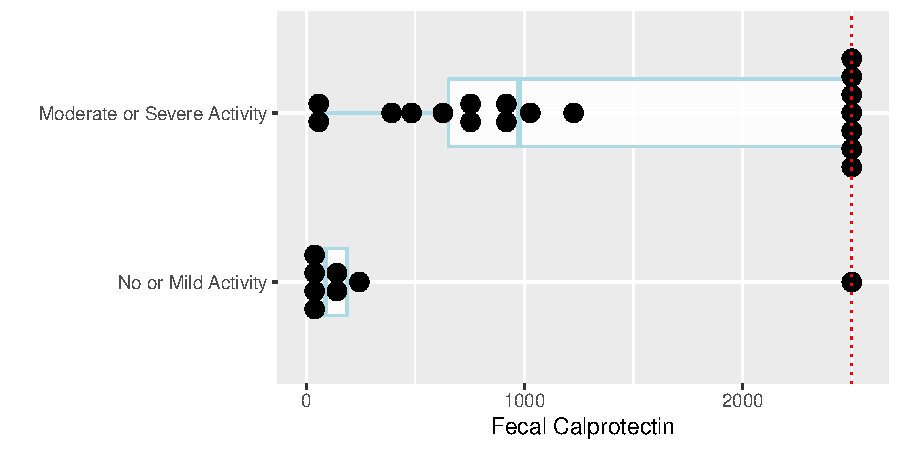
\includegraphics[width=\maxwidth]{nonpar-calpro-1} }

\caption[Fecal calprotectin by severity]{Fecal calprotectin by endoscopy severity rating. Red dotted line is the detection limit.  Ordinal disease categories should not have been combined.}\label{fig:nonpar-calpro}
\end{figure}
\end{Schunk}
% See http://docs.ggplot2.org/0.9.3/geom_dotplot.html
The following plots the ranks that are used in the
Wilcoxon-Mann-Whitney two-sample rank sum test.
\begin{Schunk}
\begin{Sinput}
ggplot(data.frame(endo, calpro), aes(y=rank(calpro), x=endo)) + #Fig (*\ref{fig:nonpar-calpror}*)
  geom_dotplot(binaxis='y', stackdir='center', position='dodge') +
    xlab('') + ylab('Rank of Fecal Calprotectin') + coord_flip()
\end{Sinput}
\begin{figure}[htbp]

\centerline{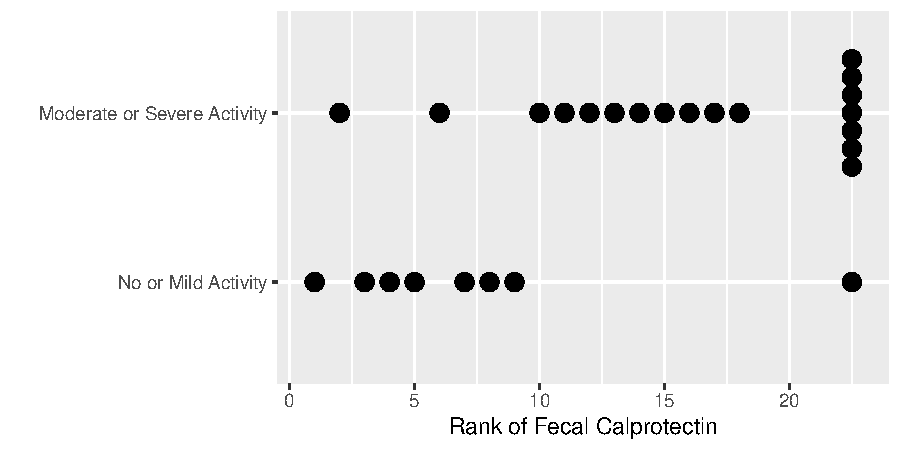
\includegraphics[width=\maxwidth]{nonpar-calpror-1} }

\caption[Ranks of calprotectin]{Ranks of calprotectin}\label{fig:nonpar-calpror}
\end{figure}
\end{Schunk}
\bi
\item Test statistic $W$ equals the sum of the ranks in the no/mild group minus $n_1 * (n_1 + 1) / 2$, where $n_1$ is the number of subjects in then no/mild sample
\item $W = 59.5 - \frac{8*9}{2} = 23.5$
\item A common (but loose) interpretation: People with moderate/severe activity have higher \textit{median} fecal calprotectin levels than people with no/mild activity ($p = 0.007$).
\item Better: remove \textit{median} and supplement with the $c$-index
  (concordance probability) or Somers' $D_{xy}$ rank correlation
  between calprotectin and endoscopy status.  The code for the \R\
  \Co{somers2} function shows how the concordance probability is
  computed from the mean of the ranks in one of the two groups.
\ei
\begin{Schunk}
\begin{Sinput}
require(Hmisc)
# Convert endo to a binary variable
somers2(calpro, endo=='Moderate or Severe Activity')
\end{Sinput}
\begin{Soutput}
         C        Dxy          n    Missing 
 0.8368056  0.6736111 26.0000000  0.0000000 
\end{Soutput}
\end{Schunk}
If you type \Co{somers2} to list the code for the function you will
see that the $c$-index is tightly related to the Wilcoxon test when
you see this code:
\begin{Schunk}
\begin{Sinput}
mean.rank <- mean(rank(x)[y == 1])
c.index <- (mean.rank - (n1 + 1)/2) / (n - n1)
\end{Sinput}
\end{Schunk}

\subsection{Point and Interval Estimates for Wilcoxon Two-Sample Comparison}
As mentioned earlier, the effect estimate that is exactly consistent
with the Wilcoxon two-sample test is the robust Hodges-Lehman estimator---the
median of all possible differences between a measurement from group 1
and a measurement from group 2.  There is a confidence interval for
this estimator.
\bi
\item Assume data come from distributions with same shape and differ only in location
\item Consider a sample of 4 males and 3 females
\item Difference in sample medians is 124 - 119.5 = 4.5
\item Consider all possible differences between sample 1 and sample 2
\ei
\begin{center}\begin{tabular}{l|cccc} \hline \hline \alabel{pg:nonpar-mf}
 & \multicolumn{4}{c}{Female} \\
Male & 120 & 118 & 121 & 119 \\ \hline
124 & 4 & 6 & 3 & 5 \\ 
120 & 0 & 2 & -1 & 1 \\
133 & 13 & 15 & 12 & 14 \\ \hline
\end{tabular}\end{center}
\bi
\item Hodges-Lehman estimate of the sex effect: median of the 12
  differences = 4.5
\item In this case equaled difference in sample medians just by coincidence
\ei
\begin{Schunk}
\begin{Sinput}
female <- c(120, 118, 121, 119)
male   <- c(124, 120, 133)
differences <- outer(male, female, '-')
differences
\end{Sinput}
\begin{Soutput}
     [,1] [,2] [,3] [,4]
[1,]    4    6    3    5
[2,]    0    2   -1    1
[3,]   13   15   12   14
\end{Soutput}
\begin{Sinput}
median(differences)
\end{Sinput}
\begin{Soutput}
[1] 4.5
\end{Soutput}
\begin{Sinput}
# Can't figure out how difference in location is computed below
# It's not the Hodges-Lehman estimate
wilcox.test(male, female, conf.int=TRUE)
\end{Sinput}
\begin{Soutput}

	Wilcoxon rank sum test with continuity correction

data:  male and female
W = 10.5, p-value = 0.1536
alternative hypothesis: true location shift is not equal to 0
95 percent confidence interval:
 -1 15
sample estimates:
difference in location 
              4.791134 
\end{Soutput}
\end{Schunk}
In general, $1 - \alpha$ confidence intervals are the set of values that if
hypothesized to be the true location parameter would not be rejected
at the $\alpha$ level.  \Co{wilcox.test} computes the location shift
by solving for the hypothesized value that yields $P=1.0$ instead of
the more proper median of all differences.  Look into this further by
plotting the $P$-value as a function of the hypothesized value.
\begin{Schunk}
\begin{Sinput}
dif  <- seq(-3, 15, by=.1)
n    <- length(dif)
pval <- numeric(n)
for(i in 1 : n) pval[i] <- wilcox.test(male - dif[i], female)$p.value
\end{Sinput}
\begin{Sinput}
ggplot(data.frame(dif, pval), aes(x=dif, y=pval)) +
  geom_step() +
  geom_hline(yintercept=.05, col='red', linetype='dotted') +
  geom_vline(xintercept=c(4.5, 4.791, -1, 15), col='red', linetype='dotted') +
  xlab('Difference') + ylab('P-value')
\end{Sinput}
\begin{figure}[htbp]

\centerline{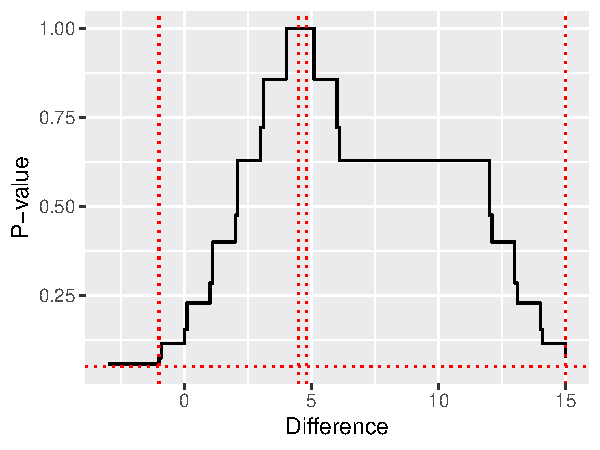
\includegraphics[width=\maxwidth]{nonpar-checkhl-1} }

\caption[Wilcoxon $P$-value vs.\ hypothesized difference.]{Wilcoxon $P$-value vs.\ hypothesized male-female difference.  Horizontal line is $P=0.05$.  Vertical lines from left to right are the lower 0.95 confidence limit from \Co{wilcox.test}, the median difference, the Hodges-Lehman estimator as computed by \Co{wilcox.test}, and the upper 0.95 confidence limit from \Co{wilcox.test}.}\label{fig:nonpar-checkhl}
\end{figure}
\end{Schunk}
See Section~\ref{sec:nonpar-clmed} for a more approximate confidence interval.

\section{Confidence Intervals for Medians and Their Differences} \altman{36-43}\alabel{sec:nonpar-clmed}
\bi 
\item Confidence intervals for the median (one sample)
\bi 
\item Table 18.4 (Altman) gives the ranks of the observations to be
  used to give approximate confidence intervals for the median 
\item e.g., if $n = 12$, the $3^\textrm{rd}$ and $10^\textrm{th}$
  largest values give a $0.961$ confidence interval 
\item For larger sample sizes, the lower ranked value ($r$) and upper
  ranked value ($s$) to select for an approximate $0.95$ confidence
  interval for the population median is 
\beq
r = \frac{n}{2} - 1.96*\frac{\sqrt{n}}{2} \hspace{.4cm}\textrm{and}
\hspace{.4cm} s = 1 + \frac{n}{2} + 1.96*\frac{\sqrt{n}}{2} 
\eeq
\item e.g., if $n = 100$ then $r = 40.2$ and $s = 60.8$, so we would pick the $40^\textrm{th}$ and $61^\textrm{st}$ largest values from the sample to specify a $0.95$ confidence interval for the population median
\item For exact confidence interval for the median see\\
  \href{https://stats.stackexchange.com/questions/186957}{stats.stackexchange.com/questions/186957}, which
  also discusses why there is no exact nonparametric confidence
  interval for the mean.  Let's get the exact order statistics that result in an exact confidence interval for the median:
\begin{Schunk}
\begin{Sinput}
# Exact CI for median from DescTools package SignTest.default
# See also ttp://www.stat.umn.edu/geyer/old03/5102/notes/rank.pdf,
# http://de.scribd.com/doc/75941305/Confidence-Interval-for-Median-Based-on-Sign-Test
cimed <- function(x, alpha=0.05, na.rm=FALSE) {
  if(na.rm) x <- x[! is.na(x)]
  n <- length(x)
  k <- qbinom(p=alpha / 2, size=n, prob=0.5, lower.tail=TRUE)
  ## Actual CL: 1 - 2 * pbinom(k - 1, size=n, prob=0.5) >= 1 - alpha
  sort(x)[c(k, n - k + 1)]
}
cimed(1 : 100)
\end{Sinput}
\begin{Soutput}
[1] 40 61
\end{Soutput}
\end{Schunk}
For $n=100$ we see that the approximate interval happened to be exact.
\ei
\item Confidence intervals for the difference in two medians (two samples)
\bi
\item We don't have a nonparametric interval for this
\item Instead get Hodges-Lehman estimate
\item Assume data come from distributions with same shape and differ only in location
\item Considers all possible differences between sample 1 and sample 2
  using male-female data on P.~\pageref{pg:nonpar-mf}
\item An estimate of the median difference (males - females) is the median of these 12 differences, with the $3^\textrm{rd}$ and $10^\textrm{th}$ largest values giving an (approximate) 0.95 CI
\item Median estimate = 4.5, 0.95 CI = [1, 13]
\item Specific formulas found in Altman, pages 40-41
\ei
\item Bootstrap \altman{159-163}
\bi
\item General method, not just for medians
\item Non-parametric, does not assume symmetry (but may not be accurate)
\item Iterative method that repeatedly samples from the original data
\item Algorithm for creating a $0.95$ CI for the difference in two medians
\begin{enumerate}
\item Sample \textit{with replacement} from sample 1 and sample 2
\item Calculate the difference in medians, save result
\item Repeat Steps 1 and 2 1000 times
\end{enumerate}
\item A (naive) $0.95$ CI is given by the $25^\textrm{th}$ and $975^\textrm{th}$ largest values of your $1000$ median differences
\item For the male/female data, median estimate = 4.5, 0.95 CI = [-0.5, 14.5], which agrees with the conclusion from a WMW rank sum test ($p = 0.15$).  Note that the more accurate CI for the Hodges-Lehman estimate of $[-1, 15]$ was given earlier (output of \co{wilcox.test}).
\ei
\ei
\begin{Schunk}
\begin{Sinput}
diffs <- numeric(1000)
set.seed(13)
for(i in 1 : 1000) diffs[i] <-
  median(sample(male, replace=TRUE)) - median(sample(female, replace=TRUE))
ggplot(data.frame(diffs), aes(x=diffs)) + xlab('Differences in Medians') +
  geom_histogram(bin_widith=.01, color='blue', fill='white')
\end{Sinput}
\begin{Sinput}
quantile(diffs, c(0.025, 0.975))
\end{Sinput}
\begin{Soutput}
 2.5% 97.5% 
 -0.5  14.5 
\end{Soutput}


\centerline{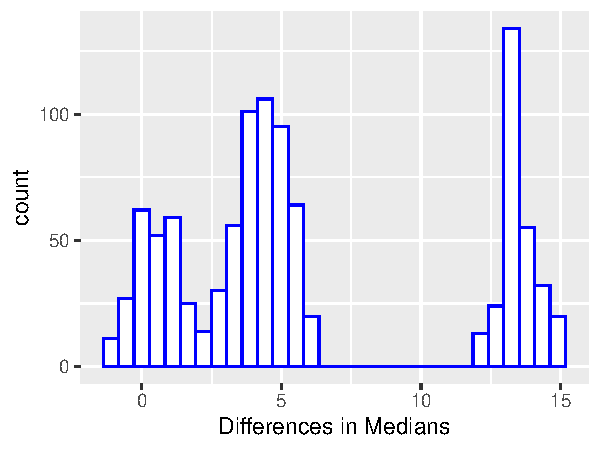
\includegraphics[width=\maxwidth]{nonpar-diffmedboot-1} }

\end{Schunk}
But recall that the Wilcoxon test does not really test the difference
in medians but rather the median of all differences.

\section{Strategy}
\bi
\item Don't assess normality of data
\item Use nonparametric test in any case, to get $P$-values
\item Use nonparametric confidence intervals for means and
  medians\footnote{A good nonparametric confidence for a population
    mean that does not even assume a symmetric distribution can be
    obtained from the bootstrap simulation procedure.}
  which will be more in conformance to what the nonpar.\ test is
  testing
\item To obtain nonparametric confidence limits for means and
  differences in means, the bootstrap percentile method may easily be
  used and it does not assume symmetry of the data distribution
\ei

\section{Generalization of the Wilcoxon/Kruskal-Wallis Test}\bmovie{11}\ddisc{11}
\bi
\item Proportional odds (PO) ordinal logistic model
\item Contains Wilcoxon 2-sample and Kruskal-Wallis tests as special cases
 \bi
 \item numerator of the score test for the PO model, when there is only the grouping variable in the model, is exactly the Wilcoxon statistic
 \ei
\item Special case of PO model is the ordinary binary logistic model
\item Advantages over nonparametric tests:
 \bi
 \item can adjust for covariates
 \item more accurate $P$-values even with extreme number of tied values
 \item provides a framework for consistent pairwise comparisons\footnote{When using the Kruskal-Wallis test followed by pairwise Wilcoxon tests, these pairwise tests can be inconsistent with each other, because they re-rank the data based only on two groups, destroying the transitivity property, e.g.\ treatment A can be better than B which is better than C but C is better than A.}
 \item provides estimates of means, quantiles, and exceedance probabilities
 \item sets the stage for a Bayesian PO model, so can get a Bayesian Wilcoxon test
 \ei
\item Other ordinal response models are available, e.g., Cox proportional hazards model
\item These models are \emph{semiparametric models}
 \bi
 \item parametric in additivity and linearity (by default) assumptions
 \item nonparametric in not assuming a distribution for the response variable
 \ei
\item Like nonparametric tests, $P$-values are unaffected by monotonic transformations of $Y$
\item If the response variable $Y$ has $k$ distinct values $y_1, y_2, \dots, y_k$ in the sample, semiparametric models have $k-1$ intercepts
\item Binary logistic model deals with prob.\ of only one event ($Y=1$ vs.\ $Y=0$)
\item For ordinal $Y$ there are $k-1$ events
\item Model these as cumulative probabilities to make use of ordering of $Y$ values
\item Model: $P(Y \geq y | X) = \frac{1}{1 + \exp[-(\alpha_y + \beta_1 x_1 + \beta_2 x_2 + \dots)]}$
\item $\alpha_y$ is the $j^{\textrm{th}}$ intercept when $y = y_{j+1}$, e.g. the first intercept corresponds to the second lowest distinct $Y$ value $y_2$
\item Special case: 2-group problem: $P(Y \geq y | \textrm{group}) = \frac{1}{1 + \exp[-(\alpha_y + \beta_1[\textrm{group B}])]}$
 \bi
 \item $\exp(\beta_1)$ is the ratio of odds that $Y \geq y$ in group B vs.\ $Y \geq y$ in group A, for all $y > y_1$ 
 \item as before $[x]$ is the 0-1 indicator variable for $x$ being true
 \item $\beta_1 > 0 \rightarrow Y$ values higher in group B
 \item $k=2 \rightarrow$ model is the binary logistic model (where we take $\alpha_1 = \beta_0$)
 \ei
\item These intercepts $\alpha_1, \alpha_2, \dots, \alpha_{k-1}$ encode the entire empirical distribution of $Y$ for one of the groups
 \bi
 \item $\rightarrow$ the model assumes nothing about the $Y$ distribution
 \item it only assumes how the distribution of $Y$ for one type of subject is connected to the distribution for another type of subject
 \item PO model for a two-group problem assumes that the logit of the two cumulative distribution functions are parallel
 \item if PO doesn't hold, PO model may still be better than alternatives
 \item PO is also what the Wilcoxon/Kruskal-Wallis test assumes to have optimal power
 \item don't need an $\alpha$ for the lowest observed $Y$ value since $P(Y \geq \textrm{minimum } Y) = 1$
 \ei
\item \R\ \co{rms} package \co{orm} function fits the PO model\footnote{\co{orm} also fits other models using link functions other than the logit.} and is especially made for continuous $Y$, with fast run times for up to 6000 intercepts
\ei

\subsection{Kruskal-Wallis Test}
\bi
\item Notice we haven't described rank ANOVA---the Kruskal-Wallis test
\item Don't need it; just form a PO model with more than one indicator variable
\item E.g., to test for any differences among four groups A B C D form 3 indicator variables for B C D and let A be the reference cell that corresponds to the $\alpha$ intercepts
 \bi
 \item model is logit$P(Y \geq y | \textrm{group}) = \alpha_y + \beta_1 [B] + \beta_2 [C] + \beta_3 [D]$
 \ei
\item Use the likelihood ratio $\chi^2$ test from this model to test the global null hypothesis A=B=C=D with 3 d.f.
\item Solves the transitivity problem mentioned earlier
\item Can obtain consistent pairwise comparisons by forming odds ratios for any comparison
 \bi
 \item e.g. C:A comparison will use $\exp(\hat{\beta_{2}})$
 \item C:B comparison OR: $\exp(\hat{\beta_{2}} - \hat{\beta_{1}})$
 \ei
\item As before can convert the ORs to differences in medians/means because unlike the original nonparametric tests, the PO model can be used to obtain many types of predictions\footnote{The predicted mean for a set of covariate settings is obtained by using all the intercepts and $\beta$s to get exceedance probabilities for $Y \geq y$, taking successive differences in those probabilities to get cell probabilities that $Y=y$, then multiplying cell probabilities by the $y$ value attached to them, and summing.  This is the formula for the mean for a discrete distribution.}
\item Illustrate this by a non-PO example, checking to see how well the PO model can recover the sample means when assuming (the slightly incorrect) PO
\item Take 4 samples from normal distributions with the same variances but different means
\item Also show how to compare two of the samples without re-ranking the data as inconsistent Wilcoxon tests would do
\ei

\begin{Sinput}
set.seed(1)
group <- rep(c('A','B','C','D'), 100)
y <- rnorm(400, 100, 15) + 10*(group == 'B') + 20*(group=='C') + 30*(group=='D')
require(rms)
options(prType='latex')
dd <- datadist(group, y); options(datadist='dd')
f <- orm(y ~ group)
f    # use LR chi-square test as replacement for Kruskal-Wallis
\end{Sinput}

 \centerline{\textbf{Logistic (Proportional Odds) Ordinal Regression Model}}
 
 \begin{verbatim}
 orm(formula = y ~ group)
 \end{verbatim}
 
 {\fontfamily{phv}\selectfont \begin{center}\begin{tabular}{|c|c|c|c|}\hline
&Model Likelihood&Discrimination&Rank Discrim.\\
&Ratio Test& Indexes&Indexes\\\hline
Obs~\hfill 400&LR $\chi^{2}$~\hfill 193.31&$R^{2}$~\hfill 0.383&$\rho$~\hfill 0.633\\
Distinct $Y$~\hfill 400&d.f.~\hfill 3&$g$~\hfill 1.532&\\
$Y_{0.5}$~\hfill 115.0935&Pr$(>\chi^{2})$~\hfill \textless 0.0001&$g_{r}$~\hfill 4.626&\\
$\max|\frac{\partial\log L}{\partial \beta}|$~\hfill $2\!\times\!10^{-6}$&Score $\chi^{2}$~\hfill 193.21&$|\overline{\mathrm{Pr}(Y\geq Y_{0.5})-\frac{1}{2}}|$~\hfill 0.256&\\
&Pr$(>\chi^{2})$~\hfill \textless 0.0001&&\\
\hline
\end{tabular}
\end{center}}
 
 %latex.default(U, file = "", first.hline.double = FALSE, table = FALSE,     longtable = TRUE, lines.page = lines.page, col.just = rep("r",         ncol(U)), rowlabel = "", already.math.col.names = TRUE,     append = TRUE)%
 \setlongtables\begin{longtable}{lrrrr}\hline
 \multicolumn{1}{l}{}&\multicolumn{1}{c}{$\hat{\beta}$}&\multicolumn{1}{c}{S.E.}&\multicolumn{1}{c}{Wald $Z$}&\multicolumn{1}{c}{Pr$(>|Z|)$}\tabularnewline
 \hline
 \endhead
 \hline
 \endfoot
 group=B&~1.4221~&~0.2579~& 5.51&\textless 0.0001\tabularnewline
 group=C&~2.6624~&~0.2762~& 9.64&\textless 0.0001\tabularnewline
 group=D&~3.6606~&~0.2925~&12.52&\textless 0.0001\tabularnewline
 \hline
 \end{longtable}
 \addtocounter{table}{-1}

\begin{Schunk}
\begin{Sinput}
# Derive R function to use all intercepts and betas to compute predicted means
M <- Mean(f)
Predict(f, group, fun=M)
\end{Sinput}
\begin{Soutput}
  group      yhat     lower    upper
1     A  99.32328  95.87128 102.8162
2     B 111.21326 108.05575 114.3752
3     C 121.63880 118.56543 124.6699
4     D 129.70290 126.48067 132.8164

Response variable (y):  

Limits are 0.95 confidence limits
\end{Soutput}
\begin{Sinput}
# Compare with sample means
summarize(y, group, smean.cl.normal)
\end{Sinput}
\begin{Soutput}
  group         y     Lower    Upper
1     A  98.72953  95.81508 101.6440
2     B 111.69464 108.61130 114.7780
3     C 121.80841 118.93036 124.6865
4     D 130.05275 127.40318 132.7023
\end{Soutput}
\begin{Sinput}
# Compare B and C
k <- contrast(f, list(group='C'), list(group='B'))
k
\end{Sinput}
\begin{Soutput}
   Contrast      S.E.     Lower    Upper    Z Pr(>|z|)
11 1.240366 0.2564632 0.7377076 1.743025 4.84        0

Confidence intervals are 0.95 individual intervals
\end{Soutput}
\begin{Sinput}
# Show odds ratios instead of differences in betas
print(k, fun=exp)
\end{Sinput}
\begin{Soutput}
   Contrast S.E.    Lower    Upper    Z Pr(>|z|)
11 3.456879   NA 2.091136 5.714604 4.84        0

Confidence intervals are 0.95 individual intervals
\end{Soutput}
\end{Schunk}

\subsection{PO Re-analysis}
\bi
\item Reconsider the calprotectin data analyzed in Section~\ref{sec:calprotectin}
\item Wilcoxon: $P=0.0068, c=0.837$
\item Frequentist PO model:
{\smaller
\begin{Sinput}
require(rms)
\end{Sinput}
\begin{Sinput}
options(prType='latex')
dd <- datadist(calpro, endo); options(datadist='dd')
f <- orm(calpro ~ endo)
print(f, intercepts=TRUE)
\end{Sinput}

 \centerline{\textbf{Logistic (Proportional Odds) Ordinal Regression Model}}
 
 \begin{verbatim}
 orm(formula = calpro ~ endo)
 \end{verbatim}
 
 
 \centerline{Frequencies of Responses}
 
 \begin{verbatim}
   18   30   38   57   61   86  114  168  244  392  483  627  726  781  910  925 
    1    1    1    1    1    1    1    1    1    1    1    1    1    1    1    1 
 1027 1226 2500 
    1    1    8 
 \end{verbatim}
 
 {\fontfamily{phv}\selectfont \begin{center}\begin{tabular}{|c|c|c|c|}\hline
&Model Likelihood&Discrimination&Rank Discrim.\\
&Ratio Test& Indexes&Indexes\\\hline
Obs~\hfill 26&LR $\chi^{2}$~\hfill 9.84&$R^{2}$~\hfill 0.317&$\rho$~\hfill 0.547\\
Distinct $Y$~\hfill 19&d.f.~\hfill 1&$g$~\hfill 1.222&\\
$Y_{0.5}$~\hfill 726&Pr$(>\chi^{2})$~\hfill 0.0017&$g_{r}$~\hfill 3.395&\\
$\max|\frac{\partial\log L}{\partial \beta}|$~\hfill $5\!\times\!10^{-5}$&Score $\chi^{2}$~\hfill 9.86&$|\overline{\mathrm{Pr}(Y\geq Y_{0.5})-\frac{1}{2}}|$~\hfill 0.251&\\
&Pr$(>\chi^{2})$~\hfill 0.0017&&\\
\hline
\end{tabular}
\end{center}}
 
 %latex.default(U, file = "", first.hline.double = FALSE, table = FALSE,     longtable = TRUE, lines.page = lines.page, col.just = rep("r",         ncol(U)), rowlabel = "", already.math.col.names = TRUE,     append = TRUE)%
 \setlongtables\begin{longtable}{lrrrr}\hline
 \multicolumn{1}{l}{}&\multicolumn{1}{c}{$\hat{\beta}$}&\multicolumn{1}{c}{S.E.}&\multicolumn{1}{c}{Wald $Z$}&\multicolumn{1}{c}{Pr$(>|Z|)$}\tabularnewline
 \hline
 \endhead
 \hline
 \endfoot
 y$\geq$30&~ 2.0969~&~1.0756~& 1.95&0.0512\tabularnewline
 y$\geq$38&~ 1.3395~&~0.8160~& 1.64&0.1007\tabularnewline
 y$\geq$57&~ 0.8678~&~0.7135~& 1.22&0.2239\tabularnewline
 y$\geq$61&~ 0.4733~&~0.6689~& 0.71&0.4792\tabularnewline
 y$\geq$86&~ 0.1122~&~0.6575~& 0.17&0.8645\tabularnewline
 y$\geq$114&~-0.1956~&~0.6558~&-0.30&0.7655\tabularnewline
 y$\geq$168&~-0.4710~&~0.6608~&-0.71&0.4760\tabularnewline
 y$\geq$244&~-0.7653~&~0.6868~&-1.11&0.2652\tabularnewline
 y$\geq$392&~-1.0953~&~0.7427~&-1.47&0.1403\tabularnewline
 y$\geq$483&~-1.4155~&~0.8015~&-1.77&0.0774\tabularnewline
 y$\geq$627&~-1.6849~&~0.8383~&-2.01&0.0445\tabularnewline
 y$\geq$726&~-1.9227~&~0.8641~&-2.23&0.0261\tabularnewline
 y$\geq$781&~-2.1399~&~0.8836~&-2.42&0.0154\tabularnewline
 y$\geq$910&~-2.3439~&~0.8993~&-2.61&0.0092\tabularnewline
 y$\geq$925&~-2.5396~&~0.9128~&-2.78&0.0054\tabularnewline
 y$\geq$1027&~-2.7312~&~0.9249~&-2.95&0.0031\tabularnewline
 y$\geq$1226&~-2.9224~&~0.9365~&-3.12&0.0018\tabularnewline
 y$\geq$2500&~-3.1166~&~0.9482~&-3.29&0.0010\tabularnewline
 endo=Moderate or Severe Activity&~ 2.7586~&~0.9576~& 2.88&0.0040\tabularnewline
 \hline
 \end{longtable}
 \addtocounter{table}{-1}

}
\item Intercept -3.1166 corresponds $Y$ being at or above the upper detection limit
\item Use the likelihood ratio (LR) $\chi^2$ test from the model
\item To estimate an exceedance probability just select the corresponding intercept and compute as for a binary logistic model
\item The 18 intercepts for 19 distinct $Y$ values represent the logit of the empirical cumulative distribution function for the no/mild reference group if the two groups are in proportional odds\footnote{The intercepts really represent the logit of one minus the CDF, moved one $Y$ value.}.  Add 2.7586 to those intercepts to get the logit CDF for the moderate/severe group.
\item Compute odds ratio and CI
{\smaller[2]
\begin{Sinput}
summary(f, endo='No or Mild Activity')
\end{Sinput}
%latex.default(cstats, caption = if (table.env) caption else NULL,     title = title, rowlabel = "", col.just = rep("r", 7), table.env = table.env,     ...)%
\begin{center}
\begin{tabular}{lrrrrrrr}
\hline\hline
\multicolumn{1}{l}{}&\multicolumn{1}{c}{Low}&\multicolumn{1}{c}{High}&\multicolumn{1}{c}{$\Delta$}&\multicolumn{1}{c}{Effect}&\multicolumn{1}{c}{S.E.}&\multicolumn{1}{c}{Lower 0.95}&\multicolumn{1}{c}{Upper 0.95}\tabularnewline
\hline
endo --- Moderate or Severe Activity:No or Mild Activity&1&2&& 2.7586&0.95757&0.88175&  4.6354\tabularnewline
~~{\it Odds Ratio}&1&2&&15.7770&&2.41510&103.0700\tabularnewline
\hline
\end{tabular}\end{center}

}
\item The above odds ratio of 15.8 is the odds of having calprotectin $\geq y$ in the moderate/severe activity group vs. the no/mild activity group
 \bi
 \item By the PO assumption this odds ratio is the same for all $y$
 \ei
\item Simulations provided an empirical conversion of the PO regression coefficient to $c$:
\begin{Schunk}
\begin{Sinput}
b <- coef(f)['endo=Moderate or Severe Activity']
cindex <- plogis((b - 0.0029) / 1.5405)
cindex
\end{Sinput}
\begin{Soutput}
endo=Moderate or Severe Activity 
                       0.8567812 
\end{Soutput}
\end{Schunk}

Compare this to the exact value of 0.837.

\item From the fitted PO model obtain for each group, compute along with sample estimates:
 \bi
 \item prob.\ calprotectin at or above the upper limit of normal
 \item mean
 \item median
 \ei
\item In the output of \co{Predict()} see the point estimates under \co{yhat}, starting with the estimates for $P(Y \geq 2500)$, i.e., marker value at or above the upper detection limit
\begin{Schunk}
\begin{Sinput}
ex <- ExProb(f)
exceed <- function(lp) ex(lp, y=2500)
ymean  <- Mean(f)
yquant <- Quantile(f)
ymed   <- function(lp) yquant(0.5, lp=lp)
Predict(f, endo, fun=exceed)
\end{Sinput}
\begin{Soutput}
                         endo       yhat       lower     upper
1         No or Mild Activity 0.04242948 0.008080776 0.1941982
2 Moderate or Severe Activity 0.41144485 0.209594428 0.6482557

Response variable (y):  

Limits are 0.95 confidence limits
\end{Soutput}
\begin{Sinput}
# Compute empirical exceedance probabilities
tapply(calpro >= 2500, endo, mean)
\end{Sinput}
\begin{Soutput}
        No or Mild Activity Moderate or Severe Activity 
                  0.1250000                   0.3888889 
\end{Soutput}
\begin{Sinput}
# Note that imposing PO assumption made modeled means closer together than
# stratified sample means
Predict(f, endo, fun=ymean)
\end{Sinput}
\begin{Soutput}
                         endo     yhat     lower     upper
1         No or Mild Activity  300.259  91.55091  851.9429
2 Moderate or Severe Activity 1387.660 895.58358 1868.2181

Response variable (y):  

Limits are 0.95 confidence limits
\end{Soutput}
\begin{Sinput}
tapply(calpro, endo, mean)
\end{Sinput}
\begin{Soutput}
        No or Mild Activity Moderate or Severe Activity 
                    400.000                    1372.944 
\end{Soutput}
\begin{Sinput}
Predict(f, endo, fun=ymed)
\end{Sinput}
\begin{Soutput}
                         endo      yhat     lower     upper
1         No or Mild Activity  69.59518  23.59636  488.0126
2 Moderate or Severe Activity 940.32171 549.13891 1653.9661

Response variable (y):  

Limits are 0.95 confidence limits
\end{Soutput}
\begin{Sinput}
tapply(calpro, endo, median)
\end{Sinput}
\begin{Soutput}
        No or Mild Activity Moderate or Severe Activity 
                       87.5                       976.0 
\end{Soutput}
\end{Schunk}
\item Note: confidence intervals for these derived quantities are approximate
\ei

\section{Checking Assumptions of the Wilcoxon Test}
\bi
\item Proportional odds (PO) model and its special case the Wilcoxon test assume PO
\item What does it mean to \emph{assume} PO?
 \bi
 \item Under $H_0$: the two distributions are \textbf{identical} there is no assumption, i.e., type I error probability will behave as advertised
 \item Under $H_1$ the test may still work OK but it will not be \emph{optimal} unless PO holds
 \ei
\item To check PO:
 \bi
 \item Compute the empirical cumulative distribution function (ECDF) for the response variable, stratified by group (see Section~\ref{sec:desc-dist})
 \item Take the logit transformation of each ECDF
 \item Check for parallelism
 \item Linearity would be required \textbf{only} if using a parametric logistic distribution instead of using our semiparametric PO model
 \ei
\item Parametric $t$-test requires parallelism \textbf{and} linearity when the ECDFs are normal-inverse transformed
  \bi
  \item linearity: normal distribution (like q-q plot)
  \item parallelism: equal variances
  \ei
\item Problem with assumption checking is that with small samples ECDFs are too noisy to see patterns clearly
\item Example from a larger dataset: Mayo Clinic Primary Biliary Cirrhosis Dataset
\item Compare distribution of serum bilirubin for those patients with spider veins vs.\ those without
\begin{Schunk}
\begin{Sinput}
getHdata(pbc)
# Take logit of ECDF
Ecdf(~ bili, group = spiders, data=pbc, fun=qlogis)
\end{Sinput}


\centerline{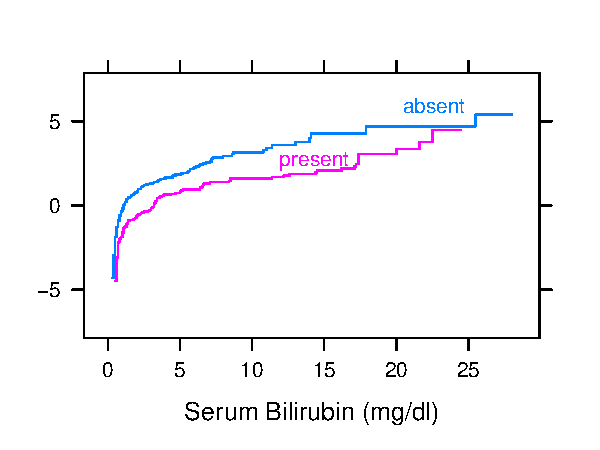
\includegraphics[width=\maxwidth]{nonpar-pbc-1} }

\end{Schunk}

\item The curves are primarily parallel (even at the far left, despite the optical illusion)
\item Nonlinearity is irrelevant
\item Check $t$-test assumptions

\begin{Schunk}
\begin{Sinput}
Ecdf(~ bili, group=spiders, data=pbc, fun=qnorm)
\end{Sinput}


\centerline{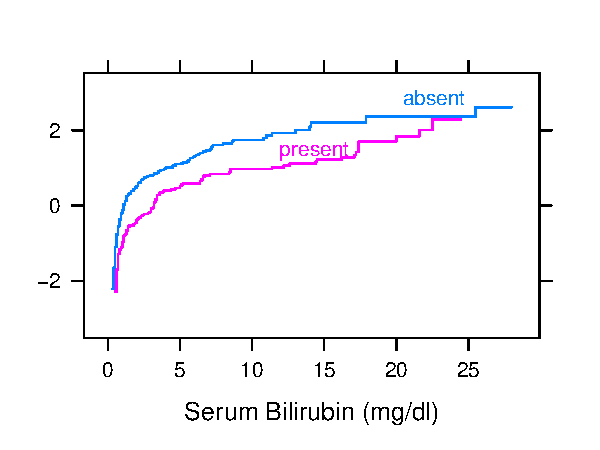
\includegraphics[width=\maxwidth]{nonpar-pbc2-1} }

\end{Schunk}
\item Curves are primarily parallel (variances are equal)
\item \textbf{But} they are not straight lines as required by $t$-test normality assumption
\ei

\section{Power and Sample Size}
\subsection{Normal Approximation}
\bi
\item Common to get power/sample size estimates for the Wilcoxon two-sample comparison using the unpaired $t$-test power formula
\item Are assuming normality and (usually) equal variances
\item To reflect the slight inefficiency of the Wilcoxon two-sample test if normality were to magically hold, multiply the $t$-test sample size by $\frac{\pi}{3} = 1.047$
\item When the response within-group distribution is far from normal this approach is suspect
 \bi
 \item e.g., $Y$ has many ties at one value, has a floor or ceiling effect, is asymmetric, or has heavy tails
 \ei
\item Need a general approach
\ei

\subsection{More on Relative Efficiency}
\bi
\item Relative efficiency of $\frac{3}{\pi}$ for the Wilcoxon 2-sample test can be derived as a correlation coefficient
\item As $n \rightarrow \infty$ it is the squared correlation between the weights Wilcoxon gives to order statistics (sorted data values) and the optimal weights
\item Wilcoxon is a \emph{linear rank statistic} with weights equal to ordinary ranks
\item Optimal linear rank test (normal scores test) for a normal distribution uses the probit link (normal inverse weights), i.e., $\Phi^{-1}(\frac{\textrm{ranks}}{n+1})$
\item Compute correlation of ordinary ranks with normal scores
\begin{Schunk}
\begin{Sinput}
for(n in c(10, 100, 1000, 10000, 100000, 1000000)) {
  ranks  <- 1 : n
  zranks <- qnorm(ranks / (n + 1))
  cat('n:', n, '  r2:', cor(ranks, zranks)^2, '\n')
}
\end{Sinput}
\begin{Soutput}
n: 10   r2: 0.9923288 
n: 100   r2: 0.9688625 
n: 1000   r2: 0.958053 
n: 10000   r2: 0.9554628 
n: 1e+05   r2: 0.955008 
n: 1e+06   r2: 0.9549402 
\end{Soutput}
\begin{Sinput}
cat('3/pi: ', 3 / pi, '\n')
\end{Sinput}
\begin{Soutput}
3/pi:  0.9549297 
\end{Soutput}
\end{Schunk}
\ei

\subsection{Tailoring Power Calculations to the Wilcoxon Test}
\bi
\item Whitehead~\cite{whi93sam} derived simple formulas related to the proportional odds model score test
\item Formulas assume that a frequency-tabulated distribution estimate is available for the combined groups
\item Power is computed as a function of the group 2 : group 1 odds ratio for exceedance probabilities
\item See example below for conversion of ORs to differences in means or medians
 \bi
 \item OR=1 $\rightarrow$ distributions are the same, so differences in means/medians are zero
 \ei
\item See \R\ \co{Hmisc} package \co{popower} and \co{posamsize} functions
\ei

\subsection{Discrete $Y$}
\bi
\item Example: response variable has clumping at zero (with prob.\ 0.3) and is otherwise uniformly distributed over the values 1, 2, 4, 8, 16, 32, 64
 \bi
 \item note: actual data values do not affect power Calculations
 \item don't come into play until translate to means/medians
 \ei
\begin{Schunk}
\begin{Sinput}
p <- c(.3, rep(.1, 7))
popower(p, 1.25, 1000)  # compute power to detect OR=1.25, combined N=1000
\end{Sinput}
\begin{Soutput}
Power: 0.516 
Efficiency of design compared with continuous response: 0.966 
\end{Soutput}
\begin{Sinput}
posamsize(p, 1.25, power=0.9)  # N for power=0.9
\end{Sinput}
\begin{Soutput}
Total sample size: 2621.4 
Efficiency of design compared with continuous response: 0.966 
\end{Soutput}
\end{Schunk}
\item Show how cell probabilities are translated by OR=1.25, and compute the mean and median of Y for a series of ORs for simpler interpretation
\begin{Schunk}
\begin{Sinput}
pomodm(p=p, odds.ratio=1.25)
\end{Sinput}
\begin{Soutput}
[1] 0.25531915 0.09250694 0.09661836 0.10101010 0.10570825 0.11074197 0.11614402
[8] 0.12195122
\end{Soutput}
\begin{Sinput}
x <- c(0, 2 ^ (0:6))
sum(p * x)  # check mean with OR=1
\end{Sinput}
\begin{Soutput}
[1] 12.7
\end{Soutput}
\begin{Sinput}
ors <- c(1, 1.05, 1.1, 1.2, 1.25, 1.5, 2)
w <- matrix(NA, nrow=length(ors), ncol=2, 
            dimnames=list(OR=ors, c('mean', 'median')))
i <- 0
for(or in ors) {
  i <- i + 1
  w[i, ] <- pomodm(x, p, odds.ratio=or)
}
w
\end{Sinput}
\begin{Soutput}
      
OR         mean   median
  1    12.70000 3.000000
  1.05 13.14602 3.364286
  1.1  13.58143 3.709091
  1.2  14.42238 4.350000
  1.25 14.82881 4.650000
  1.5  16.73559 6.000000
  2    20.03640 9.900000
\end{Soutput}
\end{Schunk}
\ei

\subsection{Gaussian $Y$}
\bi
\item Suppose response variable for control group has a normal distribution with mean 100 and SD 10
\item Start by assuming the experimental arm has the same distribution as control except with the mean shifted upwards 3 units
\item This will result in non-proportional odds so the Wilcoxon test is not optimal but will still be 0.95 efficient
\item When the sample size per group is 150, the power of the $t$-test to detect a 3-unit difference in means is:

\begin{Schunk}
\begin{Sinput}
require(pwr)
pwr.t.test(d=3 / 10, n=150, sig.level=0.05, type='two.sample')
\end{Sinput}
\begin{Soutput}

     Two-sample t test power calculation 

              n = 150
              d = 0.3
      sig.level = 0.05
          power = 0.7355674
    alternative = two.sided

NOTE: n is number in *each* group
\end{Soutput}
\end{Schunk}

\item To get the power of the Wilcoxon test when both populations have a normal distribution, we can easily use simulation

\begin{Schunk}
\begin{Sinput}
s <- 1000    # number of simulated trials
pval <- numeric(s)
set.seed(1)  # so can reproduce results
for(i in 1 : s) {
  y1 <- rnorm(150, 100, 10)
  y2 <- rnorm(150, 103, 10)
  w  <- wilcox.test(y1, y2)
  pval[i] <- w$p.value
}
mean(pval < 0.05)   # proportion of simulations with p < 0.05
\end{Sinput}
\begin{Soutput}
[1] 0.713
\end{Soutput}
\begin{Sinput}
# Simulate the power by actually running the prop. odds model 300 times
simRegOrd(300, nsim=400, delta=3, sigma=10)$power    # slower
\end{Sinput}
\begin{Soutput}
[1] 0.71
\end{Soutput}
\end{Schunk}

\item For the Wilcoxon test to be optimal (PO holds) shifting the control distribution by an odds ratio will result in a non-Gaussian distribution for the experimental arm
\item Solve for the odds ratio that shifts the mean from 100 to 103, assume PO and compute the power

\begin{Schunk}
\begin{Sinput}
# Use an arbitrary large sample to mimic population computations
m   <- 200000
y1  <- sort(rnorm(m, 100, 10))
ors <- means <- seq(1, 4, by=.025)
i   <- 0
for(or in ors) {
  i <- i + 1
  means[i] <- pomodm(y1, rep(1/m, m), odds.ratio=or)['mean']
}
plot(ors, means, xlab='Group B:A Odds Ratio',
     ylab='Mean in Population B', type='l')
abline(h=103, col=gray(.85))
needed.or <- approx(means, ors, xout=103)$y
needed.or
\end{Sinput}
\begin{Soutput}
[1] 1.708958
\end{Soutput}
\begin{Sinput}
abline(v=needed.or, col=gray(.85))
# Compute power at that odds ratio assuming no ties in data
popower(rep(1/300, 300), odds.ratio=needed.or, n=300)
\end{Sinput}
\begin{Soutput}
Power: 0.761 
Efficiency of design compared with continuous response: 1 
\end{Soutput}


\centerline{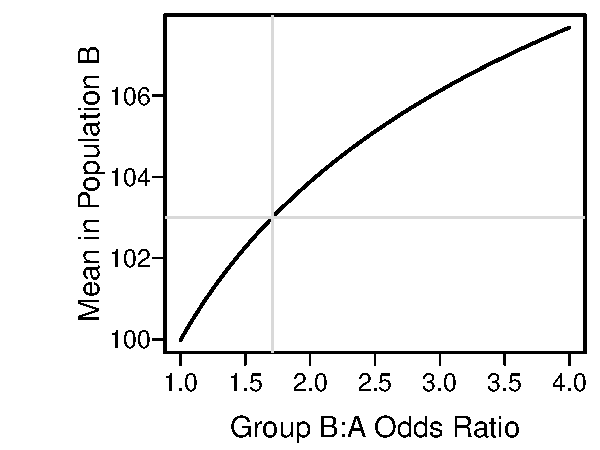
\includegraphics[width=\maxwidth]{nonpar-powerwmean-1} }

\end{Schunk}

\item Check how non-normal the experimental arm responses would be if PO holds and OR=10

\begin{Schunk}
\begin{Sinput}
# First do this theoretically
# Control arm has Gaussian Y with mean 100, SD 10
# Create experimental arm distribution using OR=10
y <- seq(60, 145, length=150)
Fy <- 1 - pnorm(y, mean=100, sd=10)    # P(Y >= y | group A)
Gy <- 1 - plogis(qlogis(Fy) + log(10)) # P(Y >= y | group B)
# Plot new CDF vs. normal approximation agreeing at quartiles
plot(y, Gy, type='l', ylab=expression(P(Y <= y)))
qu <- approx(Gy, y, xout=c(0.25, 0.5, 0.75))$y
qu    # Q1, median, Q2
\end{Sinput}
\begin{Soutput}
[1] 107.3628 113.3506 118.4894
\end{Soutput}
\begin{Sinput}
s <- (qu[3] - qu[1]) / (qnorm(0.75) - qnorm(0.25))
mu <- qu[1] - s * qnorm(0.25)
lines(y, pnorm(y, mean=mu, sd=s), col='blue')   # Gaussian fit
\end{Sinput}


\centerline{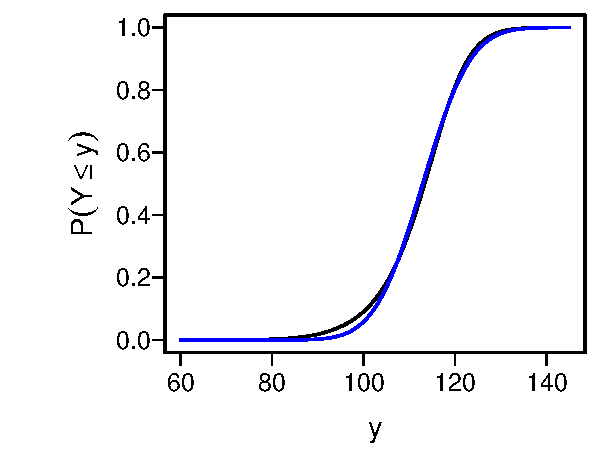
\includegraphics[width=\maxwidth]{nonpar-hownn-1} }

\end{Schunk}

\begin{Schunk}
\begin{Sinput}
# Theoretical q-q plot: check linearity of inverse normally transformed
# experimental arm distribution
plot(y, qnorm(Gy), type='l')
abline(lsfit(y, qnorm(Gy)), col='blue')
\end{Sinput}


\centerline{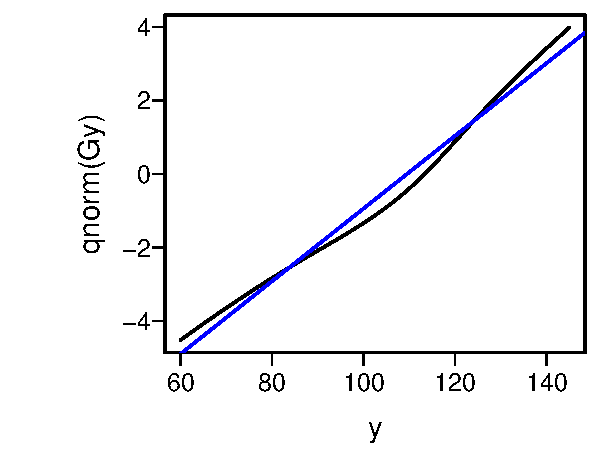
\includegraphics[width=\maxwidth]{nonpar-hownn2-1} }

\end{Schunk}

\begin{Schunk}
\begin{Sinput}
# Compute a new discrete distribution if we convert the control
# distribution using proportional odds
# Done by using a discrete distribution with 200,000 points
p <- pomodm(p=rep(1/m, m), odds.ratio=10)
range(p)  # control arm: all 1/200000
\end{Sinput}
\begin{Soutput}
[1] 5.000023e-07 4.999775e-05
\end{Soutput}
\begin{Sinput}
wtd.mean(y1, p)  # mean shifted by about 12 units
\end{Sinput}
\begin{Soutput}
[1] 112.4126
\end{Soutput}
\begin{Sinput}
# Form new distribution by repeating each observation a number
# of times equal to the ratio of the new probability to the
# minimum of all new probabilities
y2 <- rep(y1, round(p / min(p)))  # 2M obs instead of 200K
mean(y2)
\end{Sinput}
\begin{Soutput}
[1] 112.4714
\end{Soutput}
\begin{Sinput}
quantile(y2, c(.25, .5, .75))
\end{Sinput}
\begin{Soutput}
     25%      50%      75% 
107.4240 113.3446 118.5467 
\end{Soutput}
\begin{Sinput}
# The following plot is similar to the previous one
Ecdf(y2, subtitles=FALSE)
lines(y, pnorm(y, mean=mean(y2), sd=sd(y2)), col='blue')
\end{Sinput}


\centerline{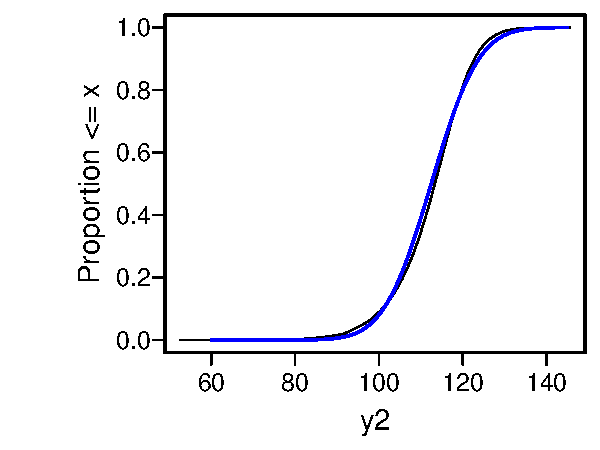
\includegraphics[width=\maxwidth]{nonpar-hownn3-1} }

\end{Schunk}

\item Little non-normality of the 2nd group if the treatment effect operates by multiplying the odds that $Y \geq y$ instead of incrementing the mean
 \bi
 \item relates to similarity of normal and logistic distributions
 \ei
\ei

\subsection{Heavy-tailed $Y$}
\bi
\item Get power to detect a shift in mean of 0.3 units for a heavy-tailed control distribution (t with 4 d.f.) with 150 subjects per group
\item Loss of efficiency of $t$-test
 \bi
 \item mean and SD are no longer optimal data summaries
 \ei
\item Can use above method to compute Wilcoxon power quickly if willing to assume PO
\item Let's not assume PO, and instead use simulation
\item Compare with power of $t$-test
\item Do for both null and non-null cases to verify type I error prob.

\begin{Schunk}
\begin{Sinput}
s <- 1000    # number of simulated trials
pvalt <- pvalw <- numeric(s)
set.seed(1)  # so can reproduce results
for(delta in c(0, 0.3)) {
  for(i in 1 : s) {
    y1 <- rt(150, 4)
    y2 <- rt(150, 4) + delta
    pvalt[i] <- t.test(y1, y2)$p.value
    pvalw[i] <- wilcox.test(y1, y2)$p.value
  }
  cat('Delta:', delta, '\n')
  P <- function(x) round(mean(x), 2)
  cat('Proportion of simulations with W p-value < t p-value:',
      P(pvalw < pvalt), '\n')
  cat('Mean p-value for t:', P(pvalt), '\n')
  cat('Mean p-value for W:', P(pvalw), '\n')
  cat('Power for t:', P(pvalt < 0.05), '\n')
  cat('Power for W:', P(pvalw < 0.05), '\n\n')
}
\end{Sinput}
\begin{Soutput}
Delta: 0 
Proportion of simulations with W p-value < t p-value: 0.51 
Mean p-value for t: 0.5 
Mean p-value for W: 0.49 
Power for t: 0.05 
Power for W: 0.06 

Delta: 0.3 
Proportion of simulations with W p-value < t p-value: 0.73 
Mean p-value for t: 0.17 
Mean p-value for W: 0.12 
Power for t: 0.47 
Power for W: 0.6 
\end{Soutput}
\end{Schunk}

\item \co{Hmisc} \co{simRegOrd} function can also simulate power for an adjusted two-sample comparison if there is one adjustment covariate
\ei

\section{Bayesian Proportional Odds Model}
\bi
\item PO model and other cumulative probability semiparametric ordinal regression models are readily extended to a Bayesian framework
\item Need special care in selecting priors for the intercepts for the continuous $Y$ case
\item Nathan James of Vanderbilt University has an implementation using Stan available at\\
\href{https://github.com/ntjames/bayes\_cpm}{github.com/ntjames/bayes\_cpm}
\item See also the \R\ \co{brms} package: \href{http://bit.ly/brms-ordinal}{bit.ly/brms-ordinal} and this discussion:\\ \href{http://github.com/paul-buerkner/brms/issues/762}{github.com/paul-buerkner/brms/issues/762}
\item Bayesian version of the Wilcoxon test is the posterior probability that $\beta_1 > 0$ in the PO model
\item Advantages of Bayes for PO models:
 \bi
 \item does not need approximations such as large sample normality of $\hat{\beta}$ or $\chi^{2}$ distribution approximation to likelihood ratio test statistic
 \item inference is more interpretable and direct
 \item can bring outside information to the analysis
 \item can incorporate shrinkage/penalization/skepticism and still have exact inference
 \item automatically obtain exact distributions and credible intervals for derived quantities\footnote{One merely takes each posterior sample for the $\alpha$s and $\beta$s and computes the quantity of interest, thereby automatically generating posterior samples for the derived quantity for which quantiles can compute credible intervals, etc.}, e.g.\ mean, quantiles, differences in means and quantiles, differences in exceedance probs, $P(Y=y | X)$
 \item can relax PO assumption without huge instabilities that result from using polytomous logistic models; prior distributions can favor PO while allowing non-PO
 \ei
\ei
